%KDD% \vspace{-1mm}
\section{Introduction}
\label{sxn:intro}

Over the past decade, Deep Neural Networks (DNNs) have proven remarkably effective on a wide range of 
computer vision (CV), natual language processing (NLP), and other domains.  
Moreover, larger and deeper DNN models, with hundreds to thousands of layers, perform tasks
seemingly impossible just a few years ago.  
For example, the CV architecture ResNet has been successfuly trained with over 1000 layers,
showing excellent generqlization performance on a wide range of data sets (CIFAR10, CIFAR100, SVHN, ImagaeNet, etc.
Most recently, openAI released the NLP Language model GPT3, which has been trained on nearly a half trillion words,
using 175 billion parameters, and achieving state-of-the-art (SOTA) performance on several NLP
benchmarks.  

The incredible size and depth of these models poses a new and deep theoretical challenges.
[blah blah blah]
Discuss Energy Landscape and  ruggedly convexity


\nred{What has been done before}

\nred{Cross Sections}
We do have some insight into how the Energy Landscape behaves by visualizing 2-dimensional
cross-sections of small models during training, such as ResNet25.
Maybe can run ourselves ?

\nred{Analysis of the Hessian}
Not really informative.  Hessian only provides local information.


\nred{Empirical Generalization Metrics}
Norm-based metrics such as WeightWatcher
Correlated with generalization / test accuracy.
Best metric is based on power law / heavy tailed.
Not explicitly data dependent



\nred{What needs to be done}
Cross-Section is not a generalization metric, is not global

Importance of unsupervised metrics: self training


In order to characterize the Energy Landscape, traditional approaches attempt to count
the number of local minima (i.e the complexity).  And while this is well for theoretical
analysis (such as spin glass theory, random matric theory, etc), numerically this
is quite hard.  Especially for the massive production size DNNs in use today.

Here, we suggest an new, alternative approach--to study the Empirical Spectral Density (ESD)
of the data-dependent Jacobian, which is readily calculated with a single epoch of Backprop
using any off-the-shelf toolkit such as TensorFlow, PyTorch, etc. 

Similar to the weightwatcher studies..

Show picture:  compare relatively random / flat vs  a deeply funneled convex Landscape ESDs

random:  real world data, randomly labeled 




Here is a summary of our main results:
\begin{itemize}
\item

\item

\item 

\end{itemize}


\paragraph{Funneled Enegy Landscapes}
\nred{where to put this ?}
\begin{figure}[h]
\begin{center}
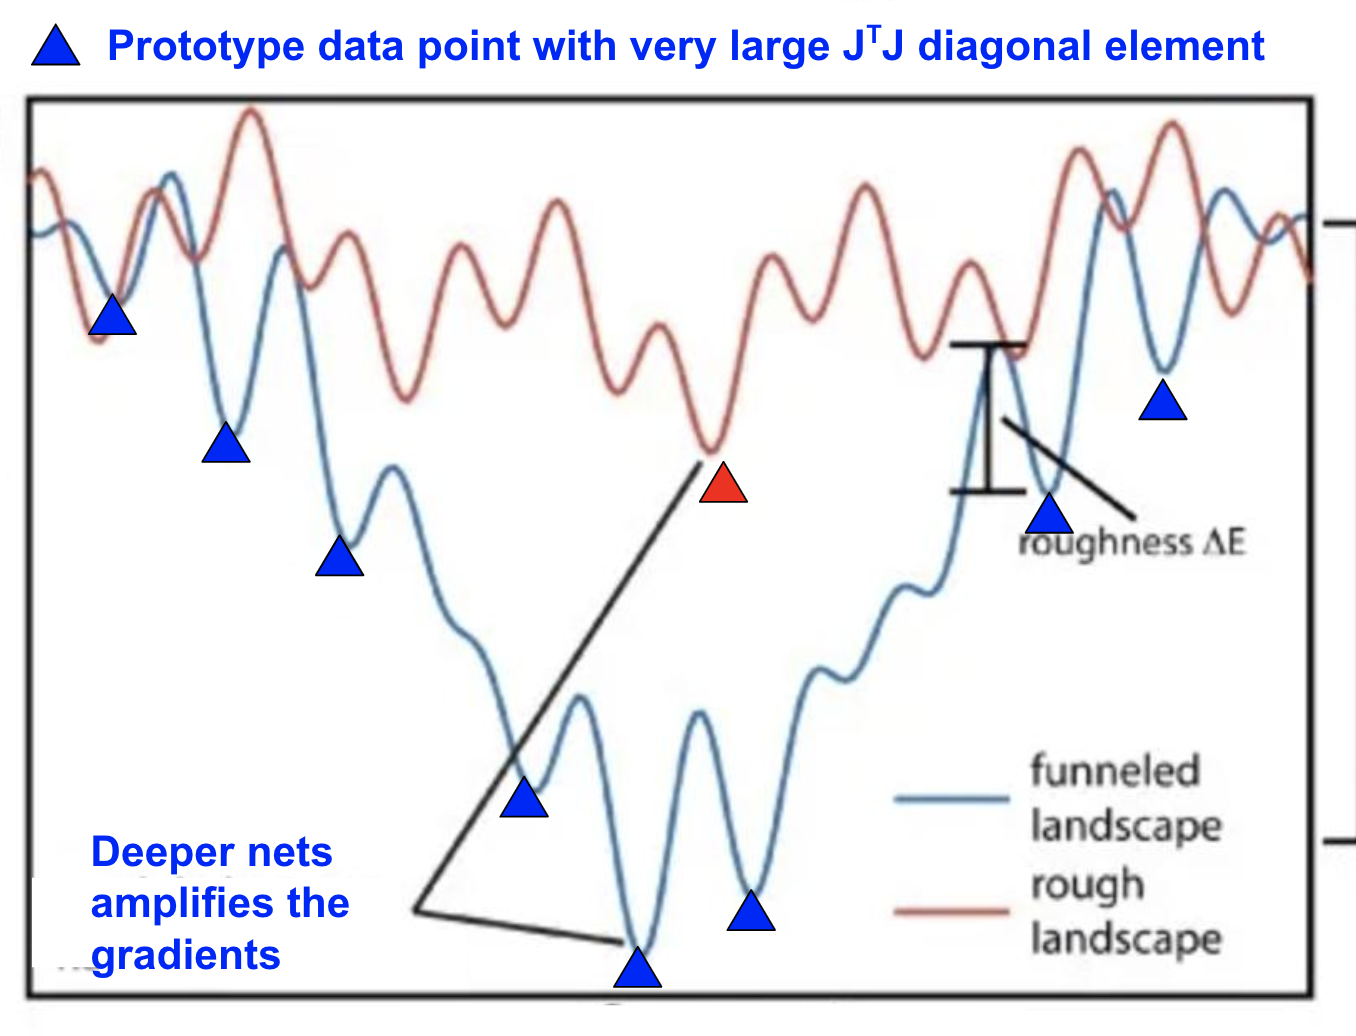
\includegraphics[scale=0.2]{img/funnel.png}
\end{center}
\caption{Sample figure caption.}
\label{fig:funnel}
\end{figure}




\paragraph{Organization of this paper.}



